\chapter{Proposed mechanisms} % for energy and performance savings

	Technique $\Rightarrow$ Benefits  \newline

1) Hardware software co-design: Re-using motion vectors generated by ISP stage to reduce the re-reference of previous image frames to calculate motion vectors for optical flow generation.\newline
(How to check if we need to compute everything with intensive vision algorithms or just use the precious results, what granularity to compute. Eg. Pyramids updating. Reactive to reconfiguration and powering on and off.)\newline
	a) Reduction of DRAM capacity requirement\newline
	b) Reduction of DRAM bandwidth requirement\newline
	c) Reducing end-to-end latency in generating dense optical flow \newline
The calculation of optical flow is the major bottleneck in terms of both memory usage and computation. The inputs for the optical flow include the current and previous camera frames of two adjacent cameras, their alpha channel and the previous optical flow. The need for temporal frames is to detect motion that is used of temporal flow regularization. Since the main memory is limited, the previous frames are usually stored in disk which increase the flow computation latency, and increase the DRAM capacity requirement and the bandwidth requirement. Instead of saving the temporal frames  for motion estimation, we can leverage the motion estimation hardware IP's that use optimal DRAM and completely remove the need to go through the disk. We model this by precomputing the motion vector and feeding with the image data. From our emulation, we found reusing the motion estimation reduces the disk utilization by \_\_ \%, the DRAM energy by \_\_ \%, improves the end-to-end latency by \_\_ \%. 
\newline

High Level Synthesis: HLS provide constructs to generate hardware that uses parallelism, pipelining, data reuse and streaming operations. On top of these we also need to do bitwidth optimization. 

2) Data driven execution: Use of motion vectors and previous optical flow to update the pyramids to make use intrinsic properties of foreground, background and motion in the scene.
	a) Reduces the number of computations 
		i) For building pyramids.
		ii) For calculating SAD(Sum of Absolute differences) during pyramid block matching.
	b) Reduces off-chip accesses
	c) Reduce end-to-end latency
\newline
Adaptive stitching pipeline *
Not all regions of the image have same level of difficulty for stitching. In an outdoor filming, most of the top portions are covered by sky, and ground is covered by road. So if those regions can be stitched with lesser effort(i.e reducing the number of iterations in stitching). Since we are going to do flow based stitching, the number of iterations is number of tiles size reductions in the flow based iterative stitching. 

3) Hardware Accelerator:
Streaming Architecture: Using raster buffers across the entire optical flow pipeline.(Number of rows is constrained by maximum motion in the scene)
a) Helpful for scalability to higher resolution
b) Reduces size of local SRAM and off-chip memory access.\newline

	\begin{tabular}{c|c|c|c}
	Power Rail & Diff. Current(mA) & Voltage(mV) & Energy ( mJ/frame) \\
	ISP+CODEC & 102.7 & 19152 & 65.6 \\
	CPU & 16.4 & 19144 & 10.5 \\
	DDR & 260.4 & 4792 & 41.6 \\
	Camera & 375.4 & 3336 & 41.7 \\
	CPU & [] & [] & [] \\
	Accelerator[Zynq] & [] & [] & [] \\
\end{tabular} \newline 


Case for low power 360 capture. Real time Stitching 30fps >4k resolution with low power. 
Latency of GPU, CPU makes them unusable for vision tasks in AR, VR.
Case for algorithm software Co-Design for a line buffer based streaming architecture. \newline

GPU Based Acceleration.
NVIDIA Tesla: A unified graphics and computing architecture. E. Lindholm, J.Nickolls, S. Oberman, and J. Montrym. IEEE HotChips 2008
The paper gives an introduction to graphics and parallel computing capabilities of Nvidia Tesla. The organization of GPU from hardware and software aspects is explained in detail. A GPU, in general, will have one or more streaming multi-processors(SMT). The SMT in Tesla consist of 8 Streaming Processor cores. The serial part of the code is implemented in CPU, whereas the Graphics and parallel computing are done in SP cores of GPU. The SM is hardware multi-threaded. It creates and executes a group of 32 threads which are of the same type of operation. They are called warps. GPU has three types of memories local global and shared. Local memory is allocated each thread and is physically located in DRAM. Shared memory is located near SMP, and used by cooperative thread arrays( thread blocks). The global memory is in DRAM and is used by sequential grids( set of blocks) to communicate large data sets. The paper also talks about CUDA programming model. In CUDA the parallelizable kernels are implemented in terms of grids and blocks and given to GPU.

1) Energy Characterization of end-to-end pipeline\newline
Camera, ISP, Computation \newline
Split of energy in computation \newline
\newline
2) Runtime Characterization \newline
a) End-to-end pipeline\newline
b) Split in computation execution\newline
\newline
3) Performing motion estimation prior to computation stage\newline
a) Savings in DRAM capacity, bandwidth(Normalized) \newline
b) Savings in DRAM Bandwidth\newline
c) Savings in overall energy\newline
d) End-to-end latency reduction\newline
\newline
4) Optimizing of computation in pyramids \newline
a) The execution time split for creation of pyramid, finding optical flow of pyramid, refining/updating the pyramids, upscaling the pyramid. \newline
98 percent is to generate optical flow(dense pixel correspondence). But only 20-30 percent actually needs to be recomputed.\newline
Main optical flow method time is 0.560256
Total time for entire optical flow is 0.584954   
 

 5) Sense the environment in gray scale and perform color mapping later? How much are you saving? 
 
 6) Egocentric motion 

7) RAM-less architecture
RAM-less architecture is possible for panoramic stitching as we plan to process data and instantly stream the processed row data from one stage to another, instead of performing computation on full image.  We need to make the computation stages generic so that it can be extended to other applications with the use of same hardware resources. We also need to work on how to program the computing units and coordinate communication between computing stages. When we generalize streaming architectures we may create idle resources in computation stages for which fine grain power gating and clock gating techniques can be used to save power from the gates that are idle. 

There can be streaming applications where the DRAM might be necessary, in such situations our architecture should be able to support the DRAM with ease. Therefore our architecture need to be flexible to include DRAM if required.

Poster data \newline
Recent advances in image sensor technology and lens designs have led to the emergence of
portable spherical panorama systems, such as the Samsung Gear 360, capturing information to
process into 360ºx180º images and videos. However, real-time, energy-efficient generation of
high-resolution spherical panoramas remains a substantial challenge, as standard
computational architectures are incapable of efficiently processing large amounts of data.
Because energy consumption generates heat, creating imaging artifacts, e.g., lens warping,
spherical panorama systems are constrained by a tight energy budget. This has led commercial
implementations to offloading-based designs, in which stitching is done on the smartphone, and
not in real-time. These implementations are incapable of scaling to large resolutions, due to
limited and energy-expensive network bandwidth. Our proposed research will create designs
that efficiently scale to ultra-high resolutions into the future, based around streaming spherical
panorama architectures that do not rely on DRAM, memory storage, or other expensive I/O
during processing. We estimate that this will create a sub-watt architecture to generate and
transmit 4K 360º video under 1 watt on the portable spherical capture device. \newline

We propose two key research goals: (i) Establish an efficient RAM-less streaming
architecture to direct fisheye sensor data into equirectangular output; and (ii) Study the effects
of early in-sensor compression to reduce the transmission of data across sensor interfaces.  \newline

\section{Stereaming feature detection and Correspondence}

We propose an architecture for feature detection and correspondence that makes effective use of spatial locality towards pixel buffers and divide-and- conquer strategies, allowing an independence from random-access memory. We expect that features detection and correspondence operations can be derived from standard corner-based algorithms, but propose to study novel hardware designs for area-efficiency and energy-efficiency. \newline

To further reduce the energy consumption of the system architecture proposed in Thrust 1, we target the image sensor physical interface as a bottleneck to energy efficiency. As temperature requirements force a substantial distance between image sensors and processing units, sensor data transactions are notoriously energy-expensive. At full input resolution of 15 MP at 30 frames per second, using a typical Low-Voltage Differential Signaling (LVDS) physical interface consumes 2W to satisfy the \&gt;3 Gbps bandwidth, e.g., [8]. This is prohibitively high, and the Gear 360 typically is constrained to capture video at one half of this available resolution, while still consuming multiple watts of average power consumption. We explore the use of in-sensor compression to assist in an energy reduction, as compared in Table 1. Existing hardware solutions for JPEG and MPEG compression are plentiful and sufficient, dropping data \newline
bitrates by substantial compression ratios (e.g., 8:1, 23:1, 46:1, etc.) and some image sensors integrate real-time JPEG encoders into their package [9]. As shown in Table 1, this can have dramatic savings on interface power consumption. Using this as our basis, Thrust 2 proposes system-oriented research for placement and utilization of compression hardware close to the sensor. Thrust 2 aims to approach research objectives of (i) processing on the compressed data, i.e., without decompression; and (ii) region-based compression quality.\newline
----------------------------------------------------


\section{High and Low Resolution combination}
What are the regions of the image frame that are needed in high resolution in order to generate a high resolution output ODS video. 
\begin{figure*}
	\begin{center}
		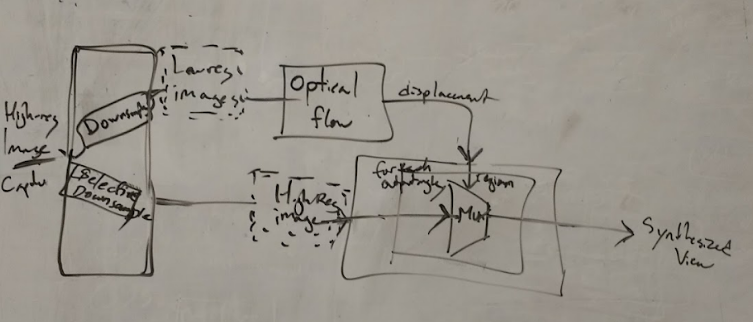
\includegraphics[width=1\textwidth]{/media/gunman/Data/thesis/ThesisLatex/data/images/HIgh_low_res_architecture.png}
		\caption{X-axis shows the pyramid level and Y-axis the runtime tile search and propagate.}
		\label{fig:ex_4_9}
	\end{center}
	\vspace{-0.3in}
\end{figure*} 








